\documentclass[graphics]{beamer}

\usepackage{graphicx}
\usepackage{verbatim}
\usepackage{wrapfig}
\useoutertheme{shadow}
%\usecolortheme{orchid}
\usecolortheme{seahorse}


% math commands
\newcommand{\be}{\begin{eqnarray}}
\newcommand{\ee}{\end{eqnarray}}
\newcommand{\beq}{\begin{equation}}
\newcommand{\eeq}{\end{equation}}
\def\simless{\mathbin{\lower 3pt\hbox
      {$\rlap{\raise 5pt\hbox{$\char'074$}}\mathchar"7218$}}}
\def\simgreat{\mathbin{\lower 3pt\hbox
      {$\rlap{\raise 5pt\hbox{$\char'076$}}\mathchar"7218$}}} %> or of order

% variables

\def\toonscale{0.45}
\def\mboxy#1{\mbox{\small #1}}


\begin{comment}
\AtBeginSection[]{
  \frame{
    \frametitle{Outline}
    \tableofcontents[currentsection]
  }
}
\end{comment}

\title{Fast radio surveys: CHIME and beyond
}
%\subtitle{interim update}
\author[U. Pen]{Ue-Li Pen, CITA/MPIfR
\\[8mm] 
}
\date{November 15, 2019}


\begin{document}

%\section*{Introduction}
\section{Current results}

\begin{comment}
  \subsection{Outline}

  \frame{
    \frametitle{Outline}
    \tableofcontents
  }
\end{comment}

\frame{\maketitle}



  \frame{
    \frametitle{FRBs}
    \begin{itemize}
        \item CHIME discovered hundreds of FRBs
        \item orders of magnitude faster discovery rate than past
          surveys
        \item coherent sources at cosmological distance: interference
          patterns, GW, lensing, etc
    \end{itemize}
%\vspace{-0.2in}
\hspace{-0.1in}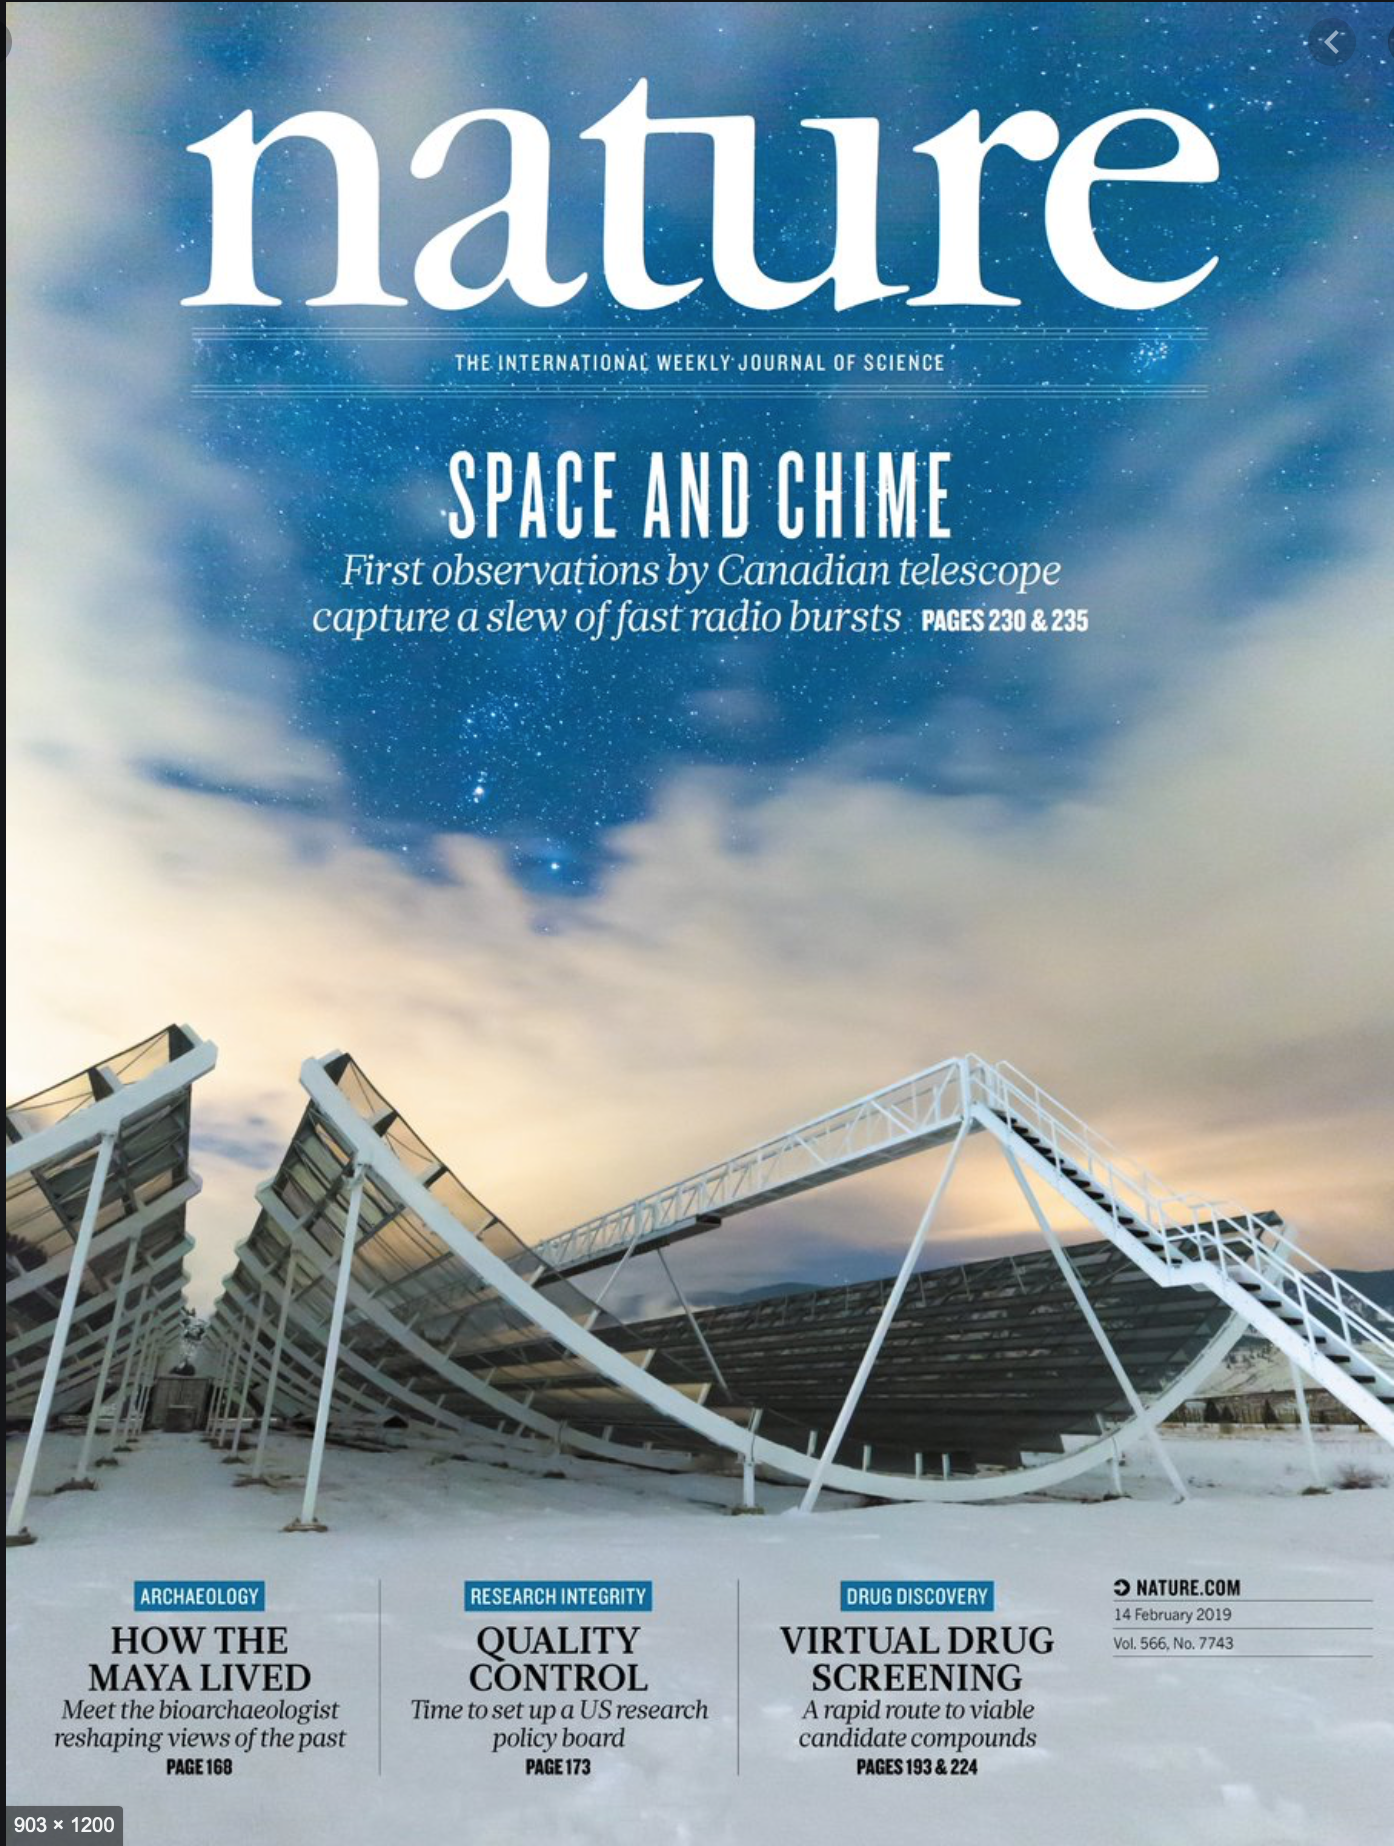
\includegraphics[width=1.6in]{Figures/chime-nature.png}
  }


  \frame{
\vspace{-0.5in}
    \frametitle{Radio Survey Science}
    \begin{itemize}
    \item CHIME history: Paris 2006+, Peterson, Ansari, Torchinski, Pittsburgh prototype++
        \item 21cm: Intensity Mapping (Chang 2008++) BAO-DE, absorbers
        \item FRB
        \item pulsar search
        \item transients: TDE, etc
        \item polarization
    \end{itemize}
  }


  \frame{
\vspace{-0.5in}
    \frametitle{Strategy}
    \begin{itemize}
        \item wide FOV
        \item large collecting area
        \item scalable processing cost
        \item FFTT!  (Tegmark\&Zaldarriaga 2009++)
        \item precision localization
    \end{itemize}
  }


  \frame{
\vspace{-0.5in}
    \frametitle{Metrics}
    \begin{itemize}
        \item flux limited survey speed: A$\Omega$
        \item time resolution: nano-sec (targeted), ms (survey)
        \item spectral resolution R=$\lambda/\Delta \lambda$: CHIME
          $\sim 10^{5-6}$
        \item dynamic range: CHIME spectral target $10^4$.
        \item trigger latency: CHIME $\sim 30$ sec
        \item localization: current $'-^o$, with outriggers $\sim$ milli-arcsec
    \end{itemize}
  }


  \frame{
\vspace{-0.5in}
    \frametitle{Algorithms}
    \begin{itemize}
        \item past telescopes: large dishes, modest number of
          receivers (ALMA $N\sim 64$)
        \item classic image forming cost $N^2$, reduce to $N\log N$
          with FFT
        \item dedispersion cost $O(n_{\rm chan}^2)$, reduce to $n \log
          n$ with tree or FFT
        \item (pulsar) periodicity search: $O([T/\tau]^2)$, again reduce to
          $\log$
        \item CHIME: $N=1024,\ n=16483,\ T/\tau\sim 10^8$
        \item scalable!
    \end{itemize}
  }



\section{Ongoing Experiments}
  \frame{
    \frametitle{CHIME}
    \begin{itemize}
        \item CHIME commissioning, first FRB's, first maps
        \item daily sky cadence, exposure time 10m-24h per pointing
    \end{itemize}
%\vspace{-0.1in}\hspace{.3in}
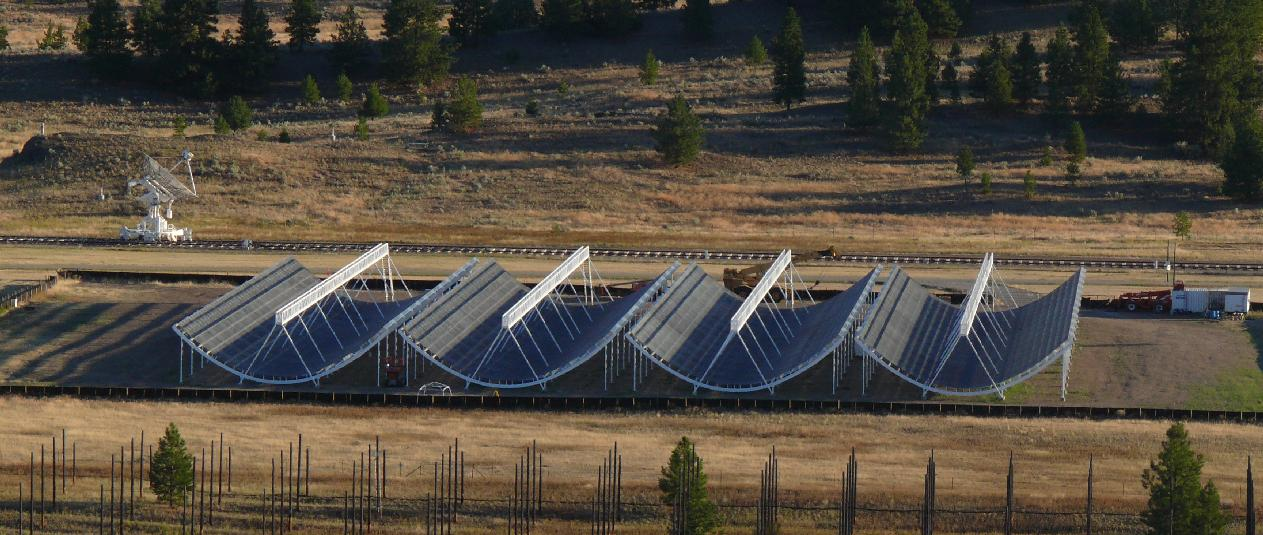
\includegraphics[width=4in]{Figures/Chime-medium.jpg}
}

  \frame{
\vspace{-0.2in}
    \frametitle{MAP}
\hspace{-0.2in}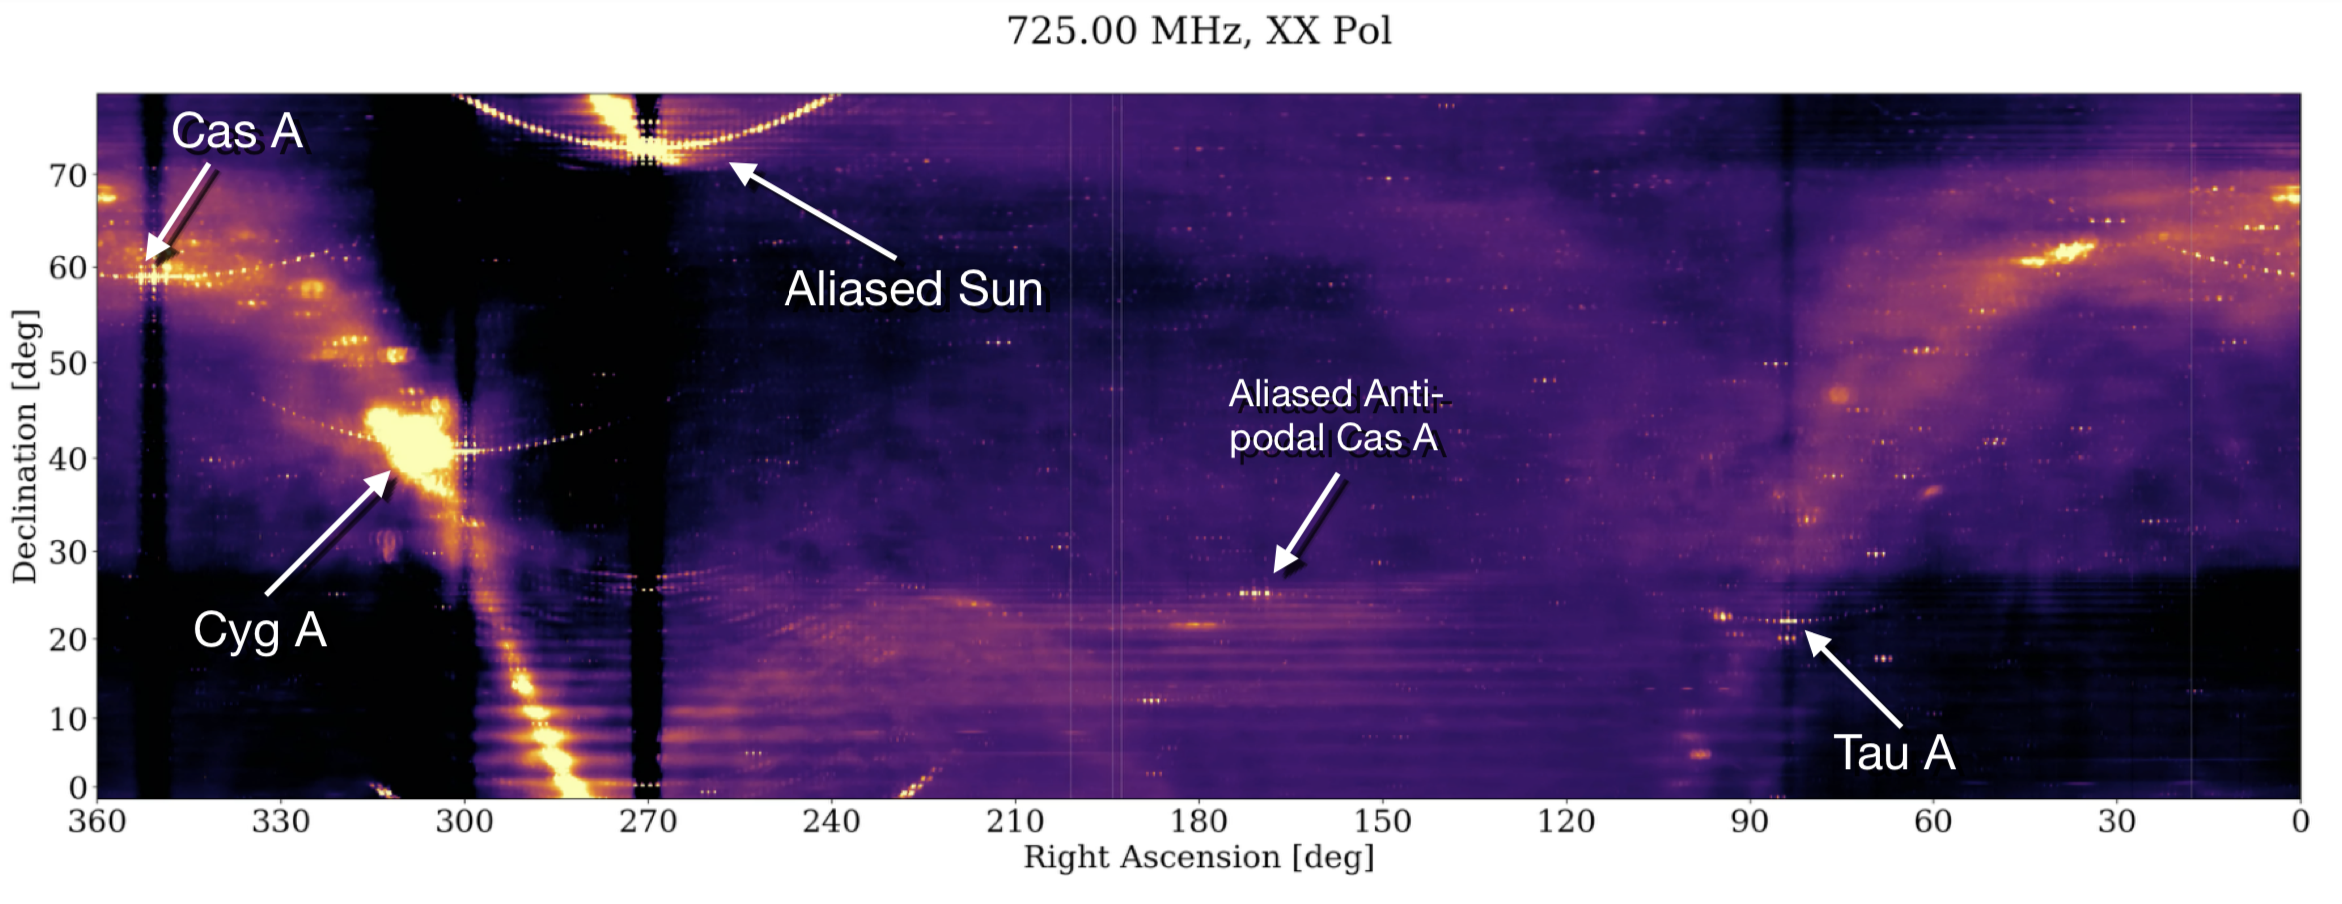
\includegraphics[width=4.5in]{Figures/CHIME-map.png}
  }

  \frame{
    \frametitle{Tianlai}
    \begin{itemize}
        \item in Xinjiang, China
        \item currently commissioning
    \end{itemize}
%\vspace{-0.1in}\hspace{.3in}
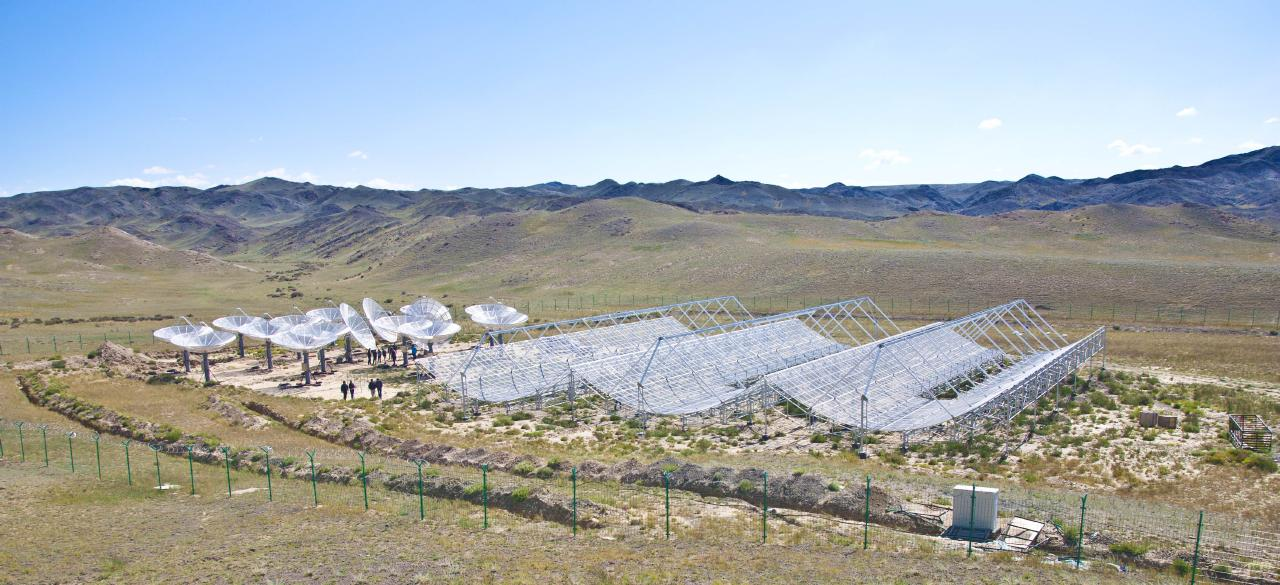
\includegraphics[width=4in]{Figures/tianlai-medium.jpg}
}

  \frame{
    \frametitle{HIRAX}
    \begin{itemize}
        \item Karoo, SA
        \item most ambitious IM-BAO project, doubles as pulsar and FRB engine
    \end{itemize}
%\vspace{-0.1in}\hspace{.3in}
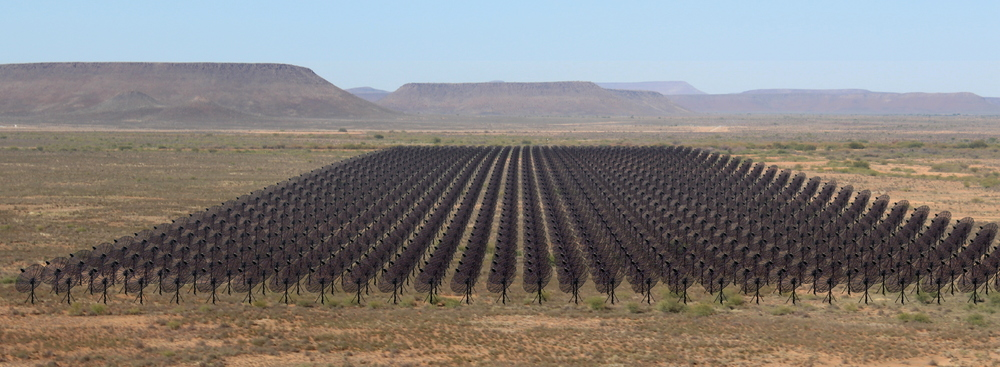
\includegraphics[width=4in]{Figures/hirax-karoo-s.jpg}
}

  \frame{
    \frametitle{Aperture Arrays}
    \begin{itemize}
        \item prototype: Nancay-EMBRACE
        \item all-sky all-time: synergy with LIGO+, GRB, $\nu$, etc
        \item ongoing discussion with MPIfR to deploy as all-sky monitor
    \end{itemize}
%\vspace{-0.1in}\hspace{.3in}
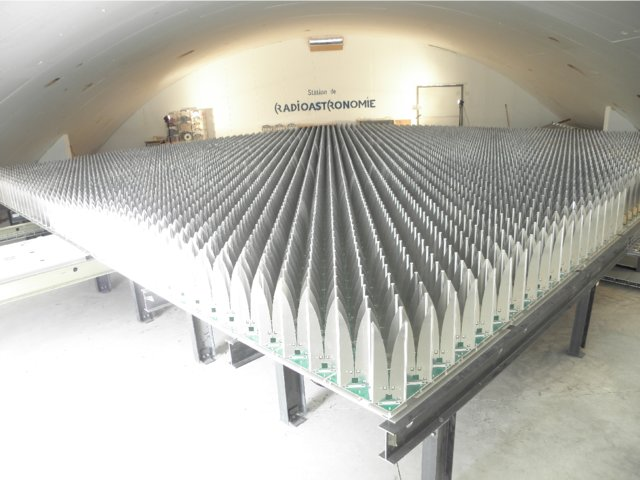
\includegraphics[width=3in]{Figures/embrace-n.jpg}
}



  \frame{
    \frametitle{Scalability}
    \begin{itemize}
        \item current CHIME cost: \$10m: $\sim \$100$ for analog chain, plus $\sim
          \$1000$/digital channel, $\$200$/m$^2$ collecting area
        \item dominated by development, primary goal speed to deployment
        \item asymptotic deployment cost likely factor of 10 lower
        \item could envision million+ element array, arbirary angular
          localization, many sq-km collecting area
        \item applications: FRB (micro-)lensing, GC binary inventory
          (Fermi-LAT connection), etc
        \item expand current sample from $\sim 10^3$ to $>10^6$
    \end{itemize}
}


  \frame{
    \frametitle{Outlook}
    \begin{itemize}
        \item CHIME first production FFTT: revolution
        \item outrigger localization in progress
        \item all-sky monitors: FFTT for aperture arrays e.g. EMBRACE
          in Nancay
        \item New potential for wide radio surveys: 21cm BAO, FRB
          cosmology
        \item FRB new potential: wave coherent source, lensing, DM, GW
    \end{itemize}
}

\end{document}
